\documentclass[a4paper, 10pt]{article}

%Internal Packages
\usepackage[utf8]{inputenc}
\usepackage[french]{babel}
\usepackage[T1]{fontenc}
\usepackage{graphicx}
\usepackage{hyperref}       % Pour les liens hypertextes

%Variables
\title{Rapport de projet : CoreWar}
\author{Amand Henry\and{}Théo Sicot\and{}Etienne Bossu\and{}Tom Rousée}
\date{\today{}}

%Document
\begin{document}
    \maketitle{}
    \newpage{}
    \tableofcontents{}
    \newpage{}

    % Introduction
    \begin{section}{Introduction} \label{sec:introduction}
        \par
            Le \textbf{Corewar} est un jeu de programmation créé en 1984 dans les universités américaines où deux programmes sont opposés pour prendre le contrôle d'une machine virtuelle appelée \textbf{MARS} (Memory Array Redcode Simulator). Ces programmes sont écrits dans un langage proche de l'assembleur appelé \textbf{RedCode}. Les programmes, appelés "Guerriers", ont pour objectif d'être les derniers à s'exécuter en faisant se terminer toutes les instances du programme adverse.
            \medskip
        \par
            Au début les joueurs concevaient leurs programmes par eux mêmes mais avec la popularisation des \textbf{algorithmes génétiques}, beaucoup utilisent l'ordinateur pour essaier de trouver les meilleurs programmes possible et gagner la partie.
            \medskip
        \par
            Ce projet était principalement tourné vers la création d'un algorithme génétique, cependant pour pouvoir le tester, il fallait créer un jeu de CoreWar complet. C'est donc ce que nous avons fait. Nous avons créé un jeu de CoreWar complet avec une machine MARS, un RedCode, un algorithme génétique et une interface graphique pour visualiser les parties.
            \medskip
        \par
            Après avoir présenté les objectifs du projet, nous allons détailler le RedCode, la machine MARS, l'algorithme génétique et l'interface graphique que nous avons créé. Nous présenterons ensuite les résultats obtenus et conclurons sur ce que nous avons appris et les perspectives d'évolution que nous pourrions mettre en place.
            \bigskip

        \begin{subsection}{Objectifs}
            \par
                L'objectif de ce projet était de créer un jeu de CoreWar complet. Pour cela nous avons dû identifier les points principaux qui composent notre projet et les implémenter. Nous avons donc décidé de découper notre projet en plusieurs parties :
                \smallskip
                \begin{enumerate}
                    \item La machine MARS
                    \item Le RedCode
                    \item Un algorithme génétique pour créer des guerriers
                    \item Une interface graphique pour afficher le déroulement des parties
                \end{enumerate}
                \medskip
                Nous avions pour la réalisation de ce projet un peu plus de 3 mois. Durée de temps appropriée car elle nous a permis de bien réfléchir aux détails de la création du jeu et de le réaliser dans les temps sans avoir a délaisser les autres cours.
                \bigskip
        \end{subsection}
    \end{section}
    

    \begin{section}{Le RedCode : Détails du Langage}
        \par
            Le \textbf{RedCode} est un langage proche de l'assembleur, uniquement utilisé par les joueurs de CoreWar et qui permet de programmer les guerriers. On utilise ce langage car par défaut il n'est pas compris par les ordinateurs. Cela évite que des personnes mal-intentionnées, ou simplement des erreurs, créent des bugs sur les pc des joueurs comme il n'y a pas risque qu'ils s'échappent de la machine MARS. Au fur et à mesure des années ce langage a évolué avec l'ajout de nouvelles instructions mais pour ce projet nous utilserons une de ses premières versions : la norme icw88 (créee een 1988). 
            
            Dans cette version, le Redcode se compose de 11 instructions. Les instructions sont des commandes qui permettent de déplacer les guerriers, de modifier la mémoire, de sauter des instructions, etc. Les opérandes sont quant à eux un couple valeur-mode qui associe un entier et le mode d'adressage de cette valeur (Direct, Indirect, Immédiat et Pre-Decrement).
            \bigskip \newline
                \textit{Voici les différentes instructions et leurs effets :}
            \bigskip

            \begin{tabular}{|c|p{8cm}|}
                \hline
                    \textbf{Instruction} & \textbf{Description} \\
                \hline
                    DAT A B & Supprime le processus en cours d'exécution de la file d'attente des processus \\
                \hline
                    MOV A B & Déplace A dans B \\
                \hline
                    ADD A B & Ajoute A à B \\
                \hline
                    SUB A B & Soustrait A à B \\
                \hline
                    JMP A B & Saute à A \\
                \hline
                    JMZ A B & Saute à A si B est égal 0\\
                \hline
                    JMN A B & Saute à A si B est différent de 0 \\
                \hline
                    CMP A B & Si A est égal à B, ignore l'instruction suivante\\
                \hline
                    SLT A B & Si A est inférieur à B, ignore l'instruction suivante\\
                \hline
                    DJN A B & Décrémente B; Si B est différent de 0, saute à A \\
                \hline
                    SPL A B & Place A dans la file d'attente des processus \\
                \hline
        \end{tabular}

        \bigskip
        Ensuite, pour définir sur quelle cellule l'instruction va s'éxécuter on retrouve 4 modes d'adressage différents. Ils sont représentés par des symboles et sont associés aux valeur A et B pour former des \textbf{Operandes}.
        \bigskip \newline
            \textit{Voici les différents modes d'adressage et leurs effets :}
        \bigskip

        \begin{tabular}{|c|p{8cm}|}
            \hline
                \textbf{Mode} & \textbf{Description} \\
            \hline
                Direct & L'opérande est une adresse mémoire vers une autre cellule \\
            \hline
                Indirect & L'opérande est une adresse mémoire vers une autre adresse (Comme si on faisait 2 Direct) \\
            \hline
                Immédiat & L'opérande est une valeur \\
            \hline
                Pre-Decrement & Similaire à l'indirect mais on fait -1 sur la deuxième adresse avant d'aller chercher la cellule \\
            \hline
        \end{tabular}

        \bigskip
        Afin de pouvoir créer des guerriers et réaliser notre projet, il est nécessaire de bien comprendre le RedCode, ses instructions et modes d'adressage. Nos premières séances furent donc dédiées a la compréhension du fonctionnement de ces derniers. Une fois compris, nous avons pu créer notre machine MARS qui interprète ces instructions et les exécute.
        \bigskip
    \end{section}




    \begin{section}{Machine MARS : Mémoire et Déroulement de la partie}
        \par
            La \textbf{machine MARS} est la pièce maitresse des parties de CoreWar. C'est la machine virtuelle dans laquelle les guerriers vont s'exécuter. Elle gère la mémoire, interprète le RedCode et est responsable du déroulement des parties, sans elle pas de projet c'est donc par là que nous avons commencé notre travail. 
            \medskip
        
        \begin{subsection}{Mémoire}
            
            \par
                Une des problèmatiques de cette partie était la \textbf{représentation de la mémoire}.
                Nous avons choisi d'utiliser une \textbf{liste doublement chainée} car la mémoire devait être circulaire et il facile de réaliser ce type de mémoire avec cette structure de données.
                \smallskip
            \par
                Dans cette liste chainée chaque cellule contient \textbf{une instruction et deux Operandes}. Pour rappel, les instructions sont les commandes que les guerriers vont exécuter et les Operandes contiennent les informations sur la méthode a appliquer pour exécuter l'instruction. 
                \medskip
            \par
                //TODO : Ajouter un UML de la mémoire
        \end{subsection}

        \begin{subsection}{Déroulement d'une partie}
            \par
                La machine MARS doit aussi gérer le déroulement de la partie. L'idée est que chaque guerrier exécute chacun à son tour une instruction. Pour cela elle a aussi à sa disposition une liste des instructions à exécuter, qui est en fait une liste de certaines cellules de la mémoire (celles dans lesquelles un guerrier à une opération en cours). Cela permet de facilement déterminer quel guerrier doit jouer et de lui faire exécuter son instruction au bon moment.
            \par
                //TODO : Process Queue / Programme et processus ?
        \end{subsection}
        \bigskip
    \end{section}



    \begin{section}{Algorithme Génétique}
        \par
            Après avoir créer la machine MARS nous avons pu développer l'algorithme génétique. L'objectif étant d'avoir un algorithme qui crée des programmes en RedCode qui sont des meilleurs guerriers que les précédent. On peut dissocier le développement de cet algorithme en deux grandes parties : Le Fonctionnement de l'algo en lui même et ensuite les différentes méthodes afin de l'entrainer efficacement.
            \medskip

        \begin{subsection}{Fonctionnement}
            \sloppypar
                Nous avons opté pour un algorithme génétique dans lequel on retrouve une grande partie d'aléatoire. Cela permet idéalement de ne pas rester bloqué sur certains programmes et d'avoir un guerrier qui est bon contre la majeure partie de ses adversaires en explorant un maximum de possibilités.
                \smallskip
            \par
                Pour cela il a d'abord fallu pouvoir générer un guerrier aléatoirement. Nous avons alors travailler sur un système de génération de \textbf{seeds} aléatoires. Ces seeds sont des nombres générés aléatoirement que l'on peut convertir en une ligne de RedCode. 
                \medskip
            \par
                \textit{\textbf{Exemple :} la ligne de RedCode "ADD @10, <5" est représenté par la ligne 02101005, 02 étant le code de l'instruction ADD, le premier 10 les modes d'adressage, puis enfin 10 et 05 les valeurs de A et B.}

        \end{subsection}

        \begin{subsection}{Entrainement}
            Description des méthodes utilisées pour l'entrainement des guerriers.

                - Le Cheatcode DAT

                - Entrainement full random

                - Le challenger

                - Population de guerriers entrainée
        \end{subsection}
    \end{section}





    \begin{section}{Interface Graphique}
        \par
            L'interface graphique permet de visualiser le déroulement des parties de CoreWar. Elle affiche la mémoire et les guerriers qui s'affrontent dedans.
            Elle se lance au choix de l'utilisateur et permet de visualiser une partie en cours. 
            \smallskip
        \par
            Toute l'interface a été faite avec le package \textbf{swing}, déjà inclus dans java. Elle transforme la mémoire en une grille. Cette grille s'adapte à toute les tailles de mémoire pour d'éventuelles parties sur une mémoire a taille réduite. Elle est composée de cases qui peuvent être de 3 couleurs différentes : Bleu, Rouge et Noir. (le Bleu et le Rouge pour chacun des guerriers et le Noir pour les cases qui n'appartiennent encore a personne).
            \bigskip
        
            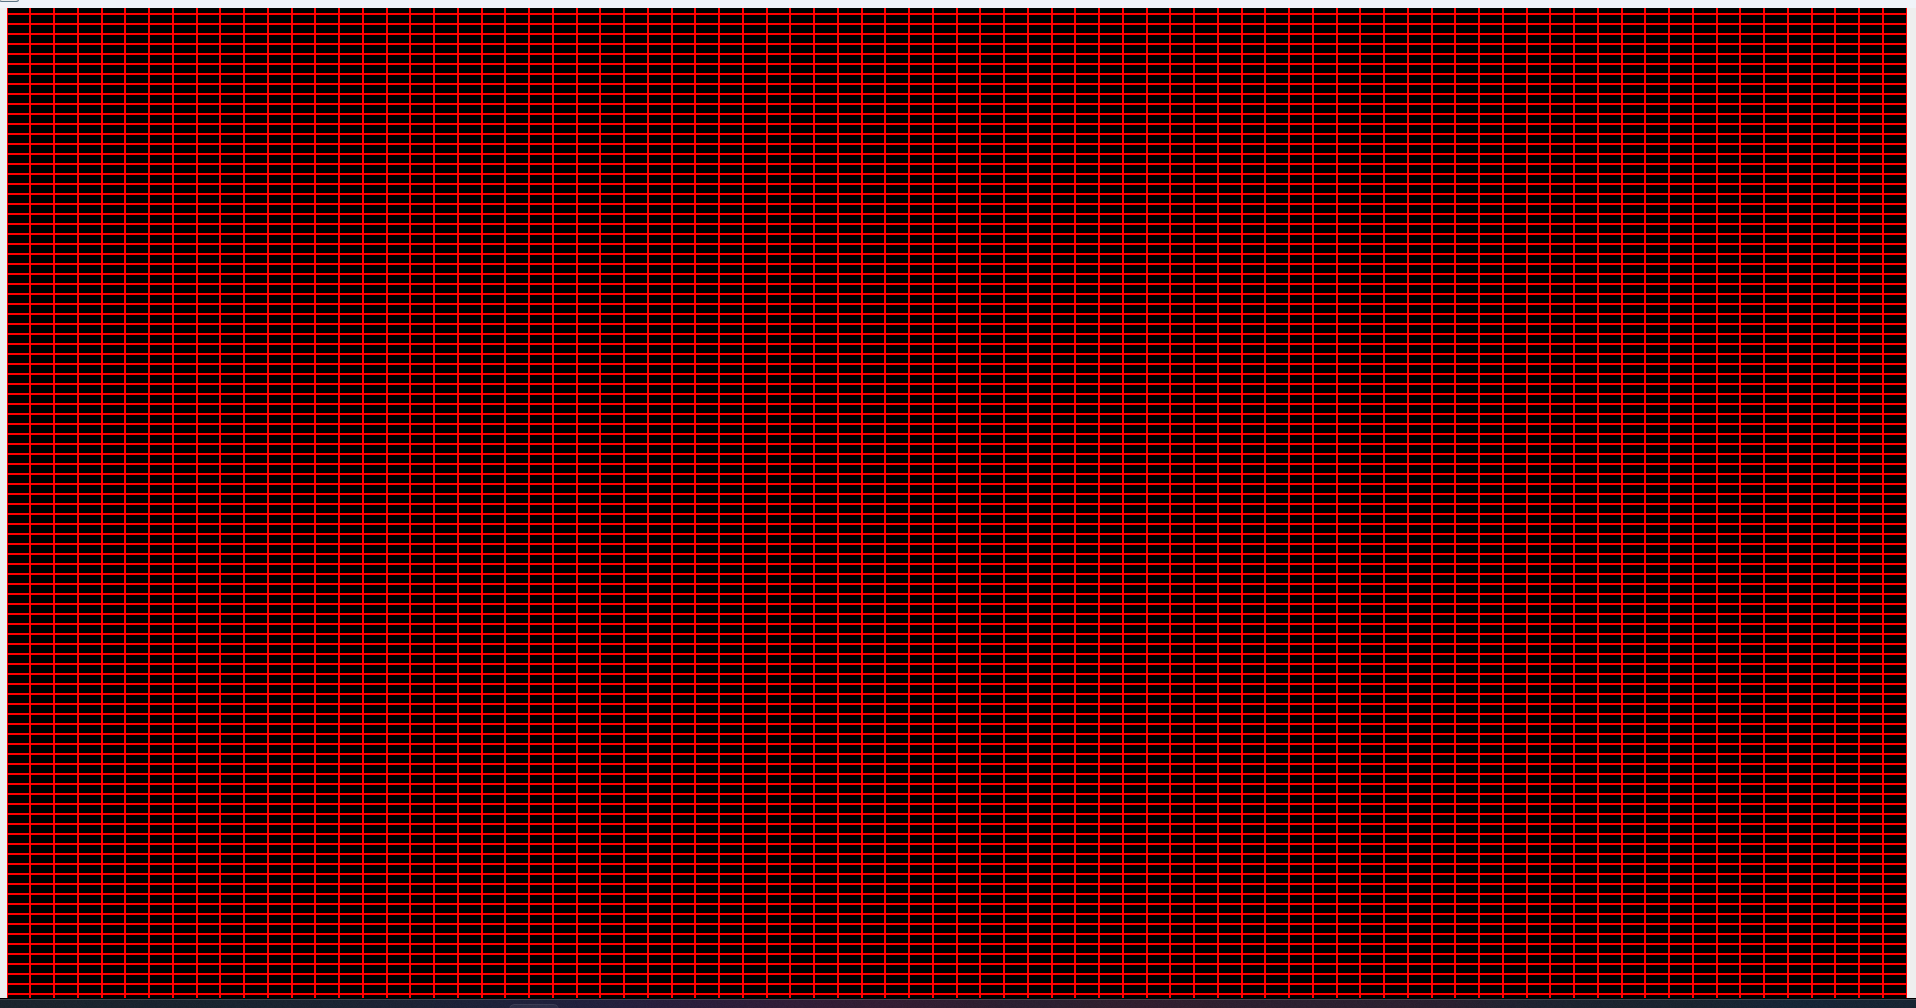
\includegraphics[width=10cm]{img/grille_interface.png}\newline
            \textit{La grille de 8000 cases, taille la plus courante pour les parties de CoreWar.}
            \bigskip

        \par
            Pour l'affichage final on efface les bordures pour afficher uniquement les couleurs. Cela permet de mieux visualiser les guerriers et de ne pas être gêné par les bordures.
            \bigskip

            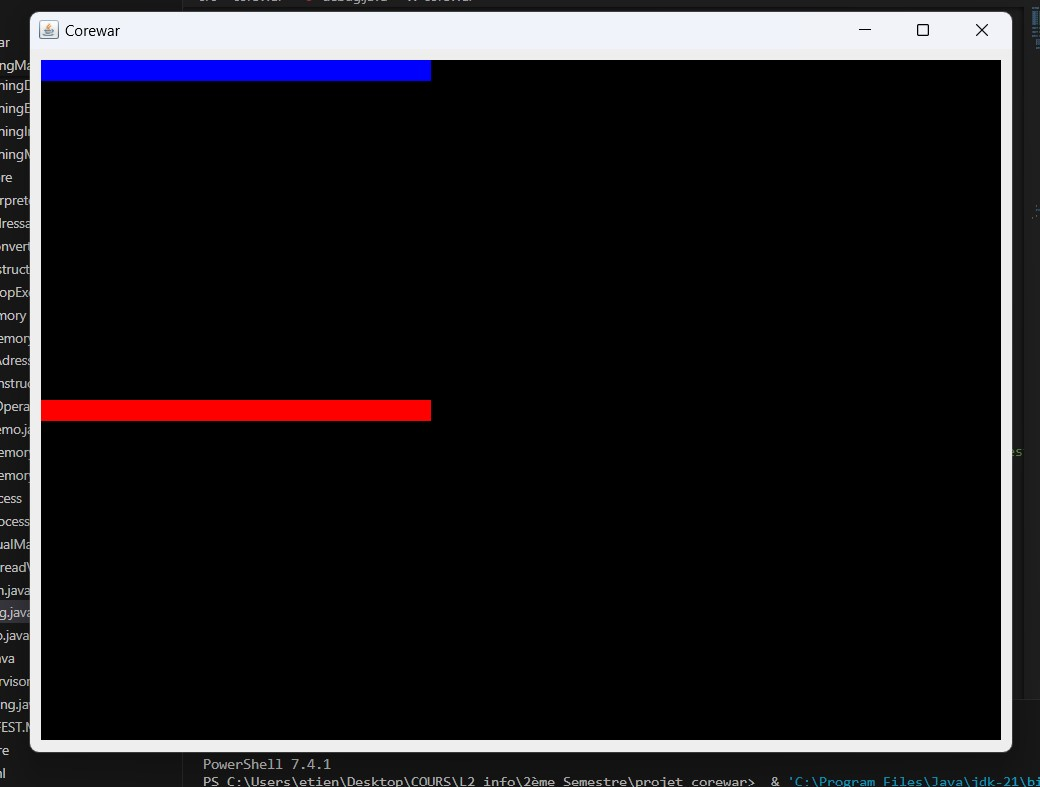
\includegraphics[width=10cm]{img/display.jpg}\newline
            \textit{Affichage final de l'interface graphique. Sans les bordures durant une partie.}
            \bigskip
        
        \par
            Pour actualiser l'affichage plusieurs méthodes ont été créées. Au départ la méthode consistait a prendre une nouvelle grille et à remplacer l'ancienne par la nouvelle. Mais cela ralentissait énormément l'affichage. Nous avons donc décidé de créer une méthode qui actualise uniquement les cases qui ont changé de couleur. Cela a permis d'optimiser l'affichage et de ne pas ralentir le jeu.
            Pour ce faire l'utilisation d'un GridBagLayout plutôt qu'un GridLayout simple a été nécessaire et il a fallu recréer l'interface. Dorénavant chaque case est gérée comme un élément indépendant et peut être actualisée indépendamment des autres.
    \end{section}

    \begin{section}{Résultats}\label{sec:resultats}
        Présentez les résultats obtenus, avec éventuellement des captures d'écran du jeu en action, des graphiques de performances, etc.
    \end{section}

    % Conclusion
    \begin{section}{Conclusion}\label{sec:conclusion}
        Résumer les résultats, ce qu'on a appris durant le projet, et les perspectives futures.
    \end{section}

    % Références
    \bibliographystyle{plain}
    \bibliography{references}
    
\end{document}